\documentclass[9pt,openany]{extbook}
\def\bleed{}

\usepackage{fontspec}
\setmainfont{EB Garamond 12 Regular}[Numbers=Lining]
\newfontfamily{\pagenfont}{Accanthis ADF Std No3}[LetterSpace=10]

\usepackage[fontset=none]{ctex}
\setCJKmainfont{Source Han Serif CN}[ItalicFont=FZKai-Z03]
\newCJKfontfamily{\sectionfont}{Source Han Serif CN Bold}
\newCJKfontfamily{\subsectionfont}{Source Han Serif CN SemiBold}
\newCJKfontfamily{\titlefont}{Source Han Serif CN Medium}
\newCJKfontfamily{\fangsong}{FZFangSong-Z02}
\newCJKfontfamily{\shusong}{FZShuSong-Z01}[ItalicFont=FZKai-Z03]

\usepackage{pifont}

\usepackage{geometry}
\geometry{
    paperwidth=6.625in,
paperheight=10.25in,
outer=10mm,
inner=5mm,
top=23mm,
headsep=5mm,
headheight=6mm,
bottom=17mm,
footskip=13mm
}

\usepackage{multicol}
\setlength{\columnseprule}{.5pt}
\setlength{\columnsep}{6.5mm}

\newcommand{\splitdot}{\shusong ·}
\newcommand{\chsline}{\hspace{0.15em}\rule[0.35em]{1.7em}{0.03em}\hspace{0.15em}}

\usepackage{titlesec}
\titleformat{\section}{\Huge\sectionfont}{}{0em}{\thispagestyle{mystyle}}
\titlespacing*{\section}{0em}{0em}{0em}
\titleformat{\subsection}{\LARGE\subsectionfont}{}{0em}{}
\titlespacing*{\subsection}{0em}{1.3em}{0.5em}

\usepackage{fancyhdr}
\renewcommand{\headrulewidth}{0pt}
\fancypagestyle{mystyle}{
    \fancyhf{}
    \fancyhead[C]{\titlefont 朱\qquad 门}
    \fancyfoot[C]{\Large\symbol{9753}\quad\pagenfont\thepage\rmfamily\quad\symbol{10087}}
}

\usepackage{graphicx}
\usepackage{float}

\usepackage{caption}
\captionsetup{
    font=small,
    labelformat=empty,
    skip=0pt,
}
\setlength{\belowcaptionskip}{-18pt}

\usepackage{indentfirst}

\usepackage{endnotes}

\renewcommand{\notesname}{\Large 注:}

\setlength{\parskip}{0em plus 1pt}

\begin{document}
\pagestyle{mystyle}
\begin{multicols}{2}
    \setcounter{page}{52}
    \begin{figure}[H]
        \centering
        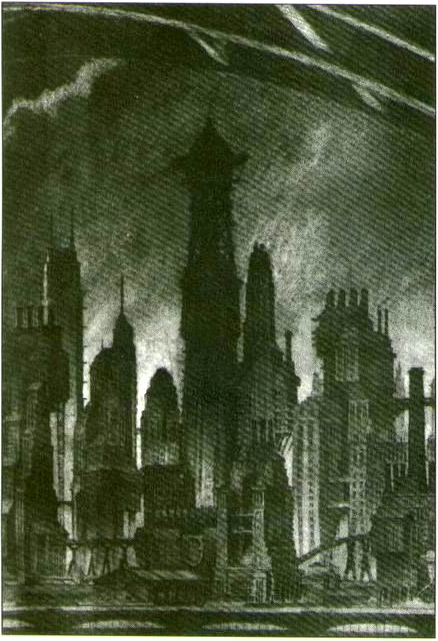
\includegraphics[width=\linewidth]{batman family history.png}
        \caption{\hfill 彼得森档案馆}
    \end{figure}

    \fangsong\noindent\LARGE\underline{书\quad 摘}\rmfamily\normalsize

    \section{巨人肩膀之上:\\哥谭背后的男人们}

    \noindent\large\textit{塞西尔{\splitdot}朗埃克著\endnote{Cecil Longacre是本文在DC宇宙内的作者。在我们的宇宙里,这篇文章是由Scott Beatty撰写的。}}\normalsize

    ~\

    \textit{作者注:}

    \textit{编撰一部哥谭的历史,这任务一看就很艰巨。当着手纪念那些字面意义上将哥谭从东北沼泽地里拽了出来{\chsline}有人称之为“连踹带嚷”地{\chsline}的男人(和女人)们时,我确实丝毫没有预料到,致富有的韦恩氏王朝的这一章中,需要回答的问题会如此之多{\chsline}答案更如此偏于推测。我研究的极早阶段,此事便相当明确。随着时间{\chsline}事实上是几百年{\chsline}的推移,关于韦恩家族的文档早已被蓄意篡改。从有法律约束的合同契约,到最私人的日记信件,在所有涉及韦恩之名的文字中,不一致之处比比皆是。以至于后文中所述的事件基本都是臆测{\chsline}确凿事实与精妙虚构间的界线从不是那么轻易就能画下的。不过,任何认知都总比没有认知要好。而真相,就在故事的字里行间等候着。}

    \noindent\large\textit{兔子草译}\normalsize

    ~\

    \textit{译者注:}

    \textit{本文中提及的近现代历史与现实中的颇有出入,原因不明。为了保留原文风貌,正文的翻译均忠于原文文意,现实历史则在注释中进行补充。}

    \subsection{第三章:韦恩们}

    大概再没哪个名字能像韦恩家族这样,与哥谭的发展和繁荣紧密相连了。

    与卡耐基\endnote{最有名的成员是Andrew Carnegie,美国历史上最有钱的人之一,在钢铁行业内举足轻重,同时也是史诗级的慈善家。}、洛克菲勒\endnote{最有名的成员是John Davison Rockefeller,也是美国历史上最有钱的人之一,石油大亨,慈善家。}或赫斯特\endnote{最有名的成员是William Randolph Hearst,美国大众媒体发展史中举足轻重的传媒大亨。}这些家族相似,自世袭财富中诞生的韦恩家也是哥谭的先驱,带领这座城市从微不足道到与美国其他伟大城市\endnote{原文为“cites”,应为“cities”的笔误。}{\chsline}纽约、芝加哥、底特律、匹兹堡\endnote{纽约与芝加哥都是哥谭的原型。“汽车之城”底特律和“钢铁之城”匹兹堡出现这里则是为了呼应哥谭“工业发达”的属性。有趣的是,此处提及的四座城市后来都在电影中出演了哥谭。《蝙蝠侠:侠影之谜》在芝加哥取景,《蝙蝠侠:黑暗骑士崛起》使用了匹兹堡和纽约,而《蝙蝠侠大战超人》则是在底特律拍摄的。}{\chsline}并列,成为举足轻重的工业圣地。

    正如所有豪门,韦恩家族与哥谭的联系也不乏奇妙之处,史实之中穿插着荒诞传闻,有的记述是平凡琐事,有的则被暗中掺入谎言。因为哥谭始于韦恩,这一点鲜少有历史学家存在异议。

    \subsection{恶人的疯人院:海兰之忏悔}

    哥谭初立时的完整年表几乎不存在,不过通过研究本地民间传言和口述历史,城市传闻的学者们得以拼凑出一段故事,将其粗略定名为“哥谭的忏悔传说”。

    尽管它读起来更像是一部道德剧,而非一份可称量的历史记录,但这段历史确实将一位不知名的韦恩列为哥谭最重要的居民之一。

    这个故事发生在十八世纪晚期,哥谭村成立的前几年。在这个相当令人不快的故事里,一个名为海兰(Hiram)的混血自由人\textit{(注:所有出版印刷的这个传说里,都没有给出过他的姓氏,使这个故事的本质更类似于寓言)}在前往布鲁德海文捕鲸定居点的路上,发现了一具横死的尸体。尽管深知这可能会归咎于他自己一样的“混种”身上,作为虔诚的宗教信徒,海兰还是在继续赶路前为这具尸体举行了基督教葬礼。然而,当到达布鲁德海文时,一个名为兰斯{\splitdot}本内迪特(Rance Benedict)的先生突然上前和海兰搭话。这是一位在捕鲸镇上很受尊敬的商人,他将自己兄弟的谋杀和失踪怪罪到海兰头上。在本内迪特的眼中,海兰的混血出身已经是最好的理由了。很自然地,海兰没承认做过任何错事。作为镇上的治安警察,本内迪特就任时就承诺了迅速执法,于是他肯定地告诉混血人海兰,他会在绞刑架上认罪。因此,海兰离开了布鲁德海文,回到了一片僻静的树林里。他曾用自己的汗水清理了这个地方,试图在此建造一座神庙。\textit{(注:一些说法不太倾向于添加“善”“恶”的角度,声称他只是在建造一个能住人的棚屋。)}

    随着故事的继续,在他回到教堂所在的路上,海兰遇到了一位神秘的“医生”,他警告海兰,有一个杀人犯正在树林区域中游荡。显然,那是个名为埃西尔帕{\splitdot}克莱文杰(Epsilpah Clevenger)的伦敦人,那位医生声称他具有不可思议的声音模仿能力,因此称之为“仿声人”。根据故事的关联性,可以认为这个“仿声人”就是兰斯{\splitdot}本内迪特兄弟凶案的真凶。随着故事发展,那位医生试图说服海兰放弃他的神庙,转而建造一座疯人院,以供东部城市里的杀人犯和纨绔浪荡子弟\endnote{原文即为将murderer与rake并列。}进行精神疗养。一场辩论接踵而至,直到两人晚上在海兰的空地上睡去,依然没有结束。

    海兰被一场可怕的暴风雨惊醒,听到了奇怪的声音。首先,那位医生大喊着说有人正在黑暗里要杀他。然后兰斯{\splitdot}本内迪特的声音从雨幕外传来,扬言他总算来报仇了。惊恐中,海兰走入倾盆大雨,拿出手枪开火,杀死了折磨他的本内迪特。但他立刻就意识到,那其实都是医生的声音模仿能力,无论是假装有人谋害他还是演绎兰斯{\splitdot}本内迪特的真正目的。后者大概确实是来为自己的兄弟复仇的,尽管没人会知道了。

    极具讽刺意味的是,那位医生揭露了他自己就是埃西尔帕{\splitdot}克莱文杰的真相,并以兰斯之死对海兰施压,说服他建造了一所疯人院,供克莱文杰和海兰自己居住。海兰轻易落入了“仿声人”的陷阱。

    海兰建造了一座疯人院,对自己、邪恶又聪明的“仿声人”埃西尔帕{\splitdot}克莱文杰、以及他的同类施以援手。虽然通常认为,这座疯人院被之后的一场大火夷为了平地。那场火灾烧焦了附近的林地,烟灰一路洒到了河流下游的布鲁德海文。但是哥谭村还是诞生了,全然不止这个定居点始于一场骗局。

    事实上,人们相信{\chsline}这大概只是一种奇妙的猜想{\chsline},哥谭当前的疗养院,阿卡姆疯人院,就建在海兰出于信仰所清理的那一块土地上。不必说,随后任何阿卡姆“闹鬼”的流言都可以直接追溯到这段历史,这场埃西尔帕{\splitdot}克莱文杰精心编织的谋杀。

    故事里的三个人哪个才是韦恩家的先祖,这个谜团仍困扰着历史学家和民俗学家们。不过,答案应该就在韦恩庄园的图书馆里,虽然直到现在,仍没有任何一个历史学家能成功混进去翻阅韦恩家族的手记和日志,来证实或否定任何理论。

    \subsection{昭示命运:所罗门{\splitdot}韦恩之智慧}

    纵然布鲁德海文是从鲸脂鲸油的恶臭中发展起来的,哥谭村却是因航运而繁荣,成为了欧洲与尚还在发展的东海岸内陆地区的交流中心。哥谭河本身就成为了南北战争前美国最重要的运河航线之一。韦恩家族在光耀门楣的路上着眼于土地收购与分割。查尔斯{\splitdot}艾文{\splitdot}韦恩(Charles Arwin Wayne)以极低廉的价格购买了数英亩的土地,其中相当一部分是沼泽地,他精明地管理了家族微薄的财产,并为他的两个儿子,所罗门{\splitdot}泽贝戴亚(Solomon Zebediah)\endnote{相关刊物\textit{Batman: Legends of the Dark Knight \#27 (1992)}。}和约书亚{\splitdot}托马斯(Joshua Thomas)\endnote{相关刊物\textit{Batman: Shadow of the Bat \#45 (1995)}。},建立了一个欣欣向荣的企业。

    查尔斯在五十二岁那年死于肺结核,而后,他的儿子们继承了他的商业遗产。许多证据都表明了所罗门对司法的热情,他“带着哈佛学位,一本法律书和一本圣经”进入哥谭村,最终成为了哥谭最年轻的,也是那个年代最杰出的联邦法官。不过,很少偶然知道所罗门的职位是因参议员纽金特{\splitdot}博尔(Nugent Bolle)的赞助获得的,那是他一位哈佛同学的父亲。

    约书亚在当时的文章里则被描述为“足够英俊,却在他火一样的法官兄弟的光辉下黯然失色”,他共同维护了几乎十几家韦恩的公司。直到,他在1860年消失得无影无踪。

    再次地,这个故事的细节相当粗糙。不过通常认为,所罗门{\splitdot}韦恩法官这位公开的废奴主义者,协助了“地下铁路(Underground Railroad)”将数不清的南方奴隶运送到加拿大获得自由之身,为他们提供安全保障的,除了韦恩家相当一部分财富,还有韦恩庄园地下的秘密交错洞窟。甚至有人认为,布里斯托镇韦恩家下方的洞窟网络,就包括在地下铁路的路径之中。

    哥谭的历史学家们更认可后一种观点,不过,地质学家们不乏敷衍地声明,布里斯托镇的岩层构成不易自然形成洞穴。或许这是历史的表态,令玩世不恭的韦恩法官显得更非同凡响。

    一些民俗学家甚至更上一层楼,将一个黑袍流氓的传说归在韦恩法官头上。这个人只用一把弯刀就击退了赏金猎人们,帮助奴隶们继续向北。然而,在1860年,约书亚{\splitdot}韦恩自哥谭失踪了。所罗门不愿对兄弟的离去做出任何评论。有人说约书亚遇到一个名为露丝(Ruth)的奴隶并爱上了她,和她一起穿过地下铁路抵达了加拿大,放弃了韦恩的财富。也有说法称韦恩回到了祖先所在的欧洲,还有一些人认为,年轻的韦恩被废奴运动深深打动,于是更名换姓,加入联邦部队对抗邦联,后来被认为阵亡于葛底斯堡。

    \subsection{补遗}

    1997年,警方记录显示在韦恩家一个酒窖地下发现了一具身份不明的骷髅,据信已有超过百年的历史。尽管没有进行刑事调查或尸检,韦恩家的家族墓地里出现了一块新碑,冠名为“约书亚{\splitdot}托马斯{\splitdot}韦恩”。唯一在世的后代,布鲁斯{\splitdot}韦恩拒绝置评。

    \subsection{美国式哥特:哥谭堡垒}

    在韦恩家所有人中,所罗门享受了最长的人生,活过了了不起的104个岁月{\chsline}长得足以看到他深爱的哥谭从朴素的村落绽放开来,他记录了从“只要不需努力,他们就惬意地如猪一样饱食终日”,到不断扩张的工业中心的演变。事实上,是所罗门{\splitdot}韦恩法官委任了备受诋毁的建筑师塞勒斯{\splitdot}平克尼(Cyrus Pinkney)\textit{(见第15章:规划者与建造者)}来设计哥谭市中心金融区散落的众多哥特式尖顶建筑。在韦恩的任命下,哥谭的标志性建筑不断发展,韦恩法官认为其与避难所或据点相差仿佛。平克尼为数不少的批评者们称,平克尼的高楼大厦只会进一步损伤哥谭的形象。尽管美国的工业化相当繁荣,但其却被诗人林肯{\splitdot}基拉维(Lincoln Killavey)描述为:“仿佛这座城市本身就是个引擎,吐出火热的空气,将烟尘与绝望倾泻在移民工人们身上。”

    纵然所罗门{\splitdot}韦恩及其后人们在经济上取得了显著成功,但布里斯托镇上韦恩庄园的空气可要比哥谭贫民窟里的甜美得多。贫民窟滋生了癌症般的犯罪。

    \subsection{韦恩的过渡岁月:禁酒令与战争}

    所罗门{\splitdot}韦恩法官去世后,家族的财富在他的儿子阿兰(Alan)的监视下继续增长。阿兰是韦恩法官的老来{\chsline}确切地说是77岁{\chsline}得子,母亲是他的第二任妻子多萝西娅(Dorothea),她比他小了近四十岁。后来,阿兰见到韦恩的土地所有权进一步在哥谭河的两岸扩张这座城市。阿兰{\splitdot}韦恩也带头发展了哥谭铁路公司,其繁复的铁路线在哥谭如今历史悠久的罗宾逊中央站交汇。借助火车头的力量,韦恩物流将许多欧洲商品运送到发展中的美国内陆,促进了韦恩企业,即家族伞形公司\endnote{一个母公司,它控股若干不同领域的子公司,整体股权结构形如一把伞,典型案例如Alphabet。}的发展。阿兰在63岁去世时,将其留给了他的儿子肯尼斯(Kenneth)。

    肯尼斯{\splitdot}韦恩,又是一位韦恩家族的精明商人,似乎预见到美国将至的“工业化”,很快会引领世界进入技术发展的时代。在肯尼斯的引导下,韦恩化工诞生了,它很快就成为了这个家族最盈利的投资之一。但与其父祖相比,肯尼斯{\splitdot}韦恩并没有那么长寿。他将韦恩的财富留给了他的遗孀劳拉{\splitdot}伊丽莎白{\splitdot}韦恩(Laura Elizabeth Wayne),她在照顾襁褓中的儿子帕特里克{\splitdot}摩根(Patrick Morgan)的同时,也展现出了敏锐的会计才华。劳拉在肯尼斯过世时仅有三十七岁,然而她终生没有再婚。与其相反,她将自己的精力集中在其他追求上。“劳拉{\splitdot}韦恩一条腿上坐着婴儿帕特里克,另一条腿上支着标牌,她对进步运动\endnote{原文仅为“the movement”,联系上下文及时代背景,应指1890s-1920s的进步运动(The Progressive Movement),概括其时政治、经济、社会领域的各种改革运动。}精神的帮助远比她自认地要多。”哥谭禁酒主义领袖珍妮{\splitdot}阿蒂克斯(Jenny Atticus)如此写道。尽管劳拉{\splitdot}韦恩的政见与哥谭许多人相左{\chsline}特别是那些仰仗废除禁酒令谋生的黑帮和私酒贩子\endnote{原文如此。现实中黑帮和私酒贩子是依靠禁酒令盈利的,文中对历史背景做出了修改,内在逻辑不明。}{\chsline},面对威胁和含沙射影的攻击,她坚韧地承受住了。如果所罗门{\splitdot}韦恩法官与她相识,一定会为此深为自豪。

    帕特里克{\splitdot}韦恩在母亲的荫蔽下成长。劳拉去世后,他继承了家族产业,带领韦恩的遗产渡过了两次世界大战\endnote{原文如此。现实中一战发生在上文提及的“进步运动”期间。},在大萧条的灰烬中重建了韦恩集团,其后是韦恩科技。战争中,它们在萨默赛特镇的飞机工厂和内维尔的造船厂为美国提供了动力,去挫败轴心国和大日本帝国的联盟\endnote{原文如此。现实中日本也是轴心国。}。

    在帕特里克{\splitdot}韦恩的领导下,韦恩之名超越了单纯哥谭的社交圈,传到更远的地方{\chsline}他将这份遗产传给了他的儿子,托马斯(Thomas)。

    \subsection{托马斯{\splitdot}韦恩:从传教到传药}

    或许世界上对未知潜力最伟大的赞歌,就是托马斯{\splitdot}韦恩的悲剧经历。正如他的祖辈们,年轻的托马斯{\splitdot}韦恩在大学毕业后壮志勃发,但却找不到一个聚焦家族潜力的方向。纵然他的父亲帕特里克{\splitdot}韦恩\endnote{原文作“父亲阿兰{\splitdot}韦恩”,显然为误。译者考虑到阿兰是托马斯的太爷爷,二人交流的可能性较低,校正为父亲帕特里克。}鼓励他进入哥谭的中心金融区学习贸易,最终掌舵家族庞大的商业帝国,可托马斯{\splitdot}韦恩却选择了离开哥谭,旅行了一段时间后,前往了加勒比海地区几个贫困小岛。

    在托马斯{\splitdot}韦恩的采访或未完成的回忆录中,并未记载他抛开奢华生活,住进小岛破屋的原因,它已失踪在时间长河中。历史学家们所知道的是,韦恩加入了一个传教士团\endnote{原文如此。现实中西班牙在大航海时代就已将天主教深入加勒比海地区,传教士在这里的工作早已结束。},致力于在小岛国家中管理人道主义援助,这些国家在疫苗接种和其他医疗支持上落后了几十年。

    韦恩在加勒比海的时间很短。当古巴军队尝试夭折的“多米诺”效应\endnote{美国总统艾森豪威尔认为,一个国家的共产主义成功将会使周边国家也倒向共产主义,称其为“多米诺理论”。只有美国叙事使用这个说法。},用共产主义团结这一地区时,除韦恩外的所有人都被杀了。不知怎的,托马斯{\splitdot}韦恩避开了抓捕,并最终回到了哥谭。令其父惊愕且失望的是,他进入了哥谭大学医学院。或许是作为传教士的经历改变了他,在父亲过世后,韦恩除了掌舵家族的经济帝国,还额外抽出时间建立了一个逐渐壮大的惯例。他将继承的大部分遗产投入了韦恩企业中,以此打造了一个慈善智囊团,它帮助了其他国家与国内外的慈善机构。

    韦恩甚至有时间追求可爱的玛莎{\splitdot}凯恩(Martha Kane),并赢得她的芳心。她是凯恩化工的唯一财产继承人,同样居住在布里斯托镇上。在哥谭的社交圈中,这被认为是一桩门当户对的婚事。然而,与这对夫妻最亲密的人{\chsline}谢天谢地,八卦新闻中并没有他们的身影{\chsline},将韦恩夫妻形容为“蒸馏提炼了真爱的精髓,并拥有其配方的专利”。

    在他们短短的十年婚姻中,玛莎生下了一个儿子,布鲁斯(Bruce)。他是独生子,他的整个人生都将被悲剧所定义。在布鲁斯快八岁时,一名枪手夺走了他双亲的生命,当时一家三口正在回家的路上。为了在哥谭的街道上散步,韦恩们给司机放了假,相当偶然地闯进了城市的阴暗一角,它甚至被市政府成为“犯罪巷”。尽管这起犯罪的记述仅仅基于警方记录和小布鲁斯接受的采访,但显然,在玛莎拒绝交出一条珍珠项链{\chsline}那是托马斯才赠给她不久的结婚纪念日礼物{\chsline}后,韦恩夫妻遭到了枪杀。托马斯试图在枪口下保护她。当时,警方困惑于为何枪手会留下幼小韦恩的活口,让他成为唯一的目击证人。托马斯{\splitdot}韦恩慈善事业的充分潜能永不会被揭晓了。再一次地,儿子继承了韦恩帝国。

    \subsection{尽头:布鲁斯{\splitdot}韦恩,乏味的花花公子}

    尽管布鲁斯{\splitdot}韦恩的早年充满悲剧,他似乎良好地度过了父母的死亡。据信,英格兰亲戚承担重任,抚养了这个孩子,让他准备好担任族长。但据说,布鲁斯{\splitdot}韦恩并没有继承哥谭历史上,他祖先们标志性的火花。布鲁斯{\splitdot}韦恩具有那种“勃发的壮志”吗?还是说,他仅仅坐下享受这个了不起的家族的余荫就已满足了?

    随着哥谭准备好进入新千禧年,人们开始好奇韦恩王朝已经走到了不可避免的终章。毕竟,所有伟大统治者的血脉,不都是终结于自己的腐朽吗?多少君王在没有继承人时就离开尘世,只因自己无能,或害怕他们的后人可能终有一日会在史书上令他们蒙羞?在这个时代,布鲁斯{\splitdot}韦恩和其他相似的人就面对着这个陷阱,富有的王子们{\chsline}即便富有程度骇人听闻的{\chsline}满大街都是。

    尽管他拥有无数荣誉,包括因帮助保护哥谭周边野生动物而成为最新的“胡蒂(Hootie)”奖获得者,布鲁斯{\splitdot}韦恩在慈善事业中花费的力气只是拿起笔签支票。尽管有人可能争辩道,韦恩的无数商业公司{\chsline}韦恩科技、韦恩化工和无可争议的慈善者韦恩企业{\chsline}的成功,确保了哥谭能继续活到下个世纪,但那会是一个没有韦恩引领着创新和进步的哥谭。对于提不起劲的布鲁斯{\splitdot}韦恩来说,他的公司显然已经是由营销天才,CEO卢修斯{\splitdot}福克斯经营的,似乎那口充分为家族效力的灵感之井终于干涸了,它服务了所罗门、劳拉{\splitdot}韦恩,甚至他自己的父亲,卓越的托马斯{\splitdot}韦恩医生。到了最后,韦恩在哥谭的遗迹只剩下了建筑与纪念碑作为标志,它们大概已经过时很久了。

    \textit{塞西尔{\splitdot}朗埃克也是《破碎的科德:泰德{\splitdot}科德\endnote{泰德{\splitdot}科德(Ted Kord),二代蓝甲虫。}的破产与崩溃》和《扎斯\endnote{扎斯(Zsasz),指维克多(Victor){\splitdot}扎斯,即扎斯先生。}风:有格调的连环凶手之自画像》的作者。}

    \theendnotes
\end{multicols}
\end{document}